\documentclass[a4paper, 12pt]{report}
\usepackage{hyperref}
\usepackage{gensymb}
\usepackage{ amssymb }
\usepackage[utf8]{inputenc} % выбор кодировки кода
\usepackage[T2A]{fontenc} % выбор внутренней кодировки 
\usepackage[english, russian]{babel} % выбор языка
\usepackage{csquotes}
% \righthyphenmin = 2 % минимальное число букв после переноса: может пригодиться
\usepackage{multirow}
\usepackage{fontawesome}
\usepackage{easyReview}
\usepackage{tabularx}
\usepackage{rotating}
\usepackage{amsmath} % русский текст в формулах
\usepackage{color} % цвет текста
\usepackage{ulem} % для зачёркивания текстаё

\usepackage[left=15mm, right=10mm, top=20mm, bottom=20mm]{geometry} % поля
\usepackage{indentfirst} % отступ первого абзаца
\setlength{\parindent}{1,25cm} % длина отступа первой строки абзаца
\linespread{1,5} % междустрочный интервал

\usepackage{titlesec} % настройка заголовков
\renewcommand{\thesection}{\arabic{section}} % противотараканная мера для report'а: делаю section заголовком первого уровня
\titleformat{\section}{\centering \large \bfseries}{\thesection}{1ex}{\MakeUppercase}{}
\titleformat{\subsection}{\centering \large \bfseries}{\thesubsection}{1ex}{}{}
\titleformat{\subparagraph}[runin]{\bfseries}{\thesubparagraph}{}{}{}

% \titleformat{\bibliography}{\centering \large \bfseries}{\thebibliography}{}{}{} % попытка настроить заголовок для списка литературы

\usepackage{graphicx}
\usepackage{wasysym}

\usepackage{comment} % Для многострочных комментариев
\usepackage{xcolor} % Для девочек 
\usepackage{enumitem} 
\usepackage{wasysym} % Для смайликов

\usepackage[
natbib		= true,
style		= gost-numeric,
sorting		= none,
backend		= biber,
language	= autobib,
bibstyle	= gost-numeric,
citestyle	= gost-numeric,
autolang	= other]{biblatex}
\addbibresource{mybiblio.bib}

\begin{document}
\begin{titlepage}
\setlength\parindent{0pt}
	\begin{center}
		\large{РОО <<Федерация спортивного туризма Московской области>>\\
		ОО г. Долгопрудного <<Федерация спортивного туризма>>\\}
	\end{center}

	


	
	\begin{center}
		\includegraphics[width=0.4\linewidth]{pics/Flag_GS-2}
		
		\Large{\bfseries{ОТЧЁТ}} \\
		\normalsize о прохождении горного спортивного туристического маршрута \textbf{первой} категории сложности по Центральному Тянь-Шаню (хребет Тескей-Ала-Тоо), совершённом с 03 по 13 августа 2025 г. группой туристов Горной секции МФТИ ФСТ Московской области, г. Долгопрудный
	\end{center}
	\vspace{1.5 cm}
	
	\textbf{Маршрутная книжка:} 55/2025, выдана МКК ФСТ МО г. Долгопрудный \\ 
	\textbf{Руководитель группы:} Остапив Алексей Юрьевич\\
	\textbf{E-mail:} \href{mailto: ostapiv\_ayu@phystech.edu}{ostapiv\_ayu@phystech.edu}\\
	\textbf{Номер телефона:} $+7(989)629-46-58$
	
	\vspace{0.2cm}
	
	\textit{Маршрутно-квалификационная комиссия Федерации спортивного туризма Московской области рассмотрела отчёт и считает, что маршрут может быть зачтен всем участникам и руководителю \textbf{первой категории сложности}.}

	\vspace{0.2cm}
	
	Отчёт использовать в библиотеке ФСТ Московской области и ФСТ г. Долгопрудный.
	
	\vspace{0.8cm}
	\textbf{Судья по виду:} 
	
%	\vspace{0.8cm}
%	\textbf{Судья по ходу:}
	
	\vspace{0.8cm}
	\textbf{Председатель МКК:}
	
	\vspace{0.8cm}
	\textbf{Штамп МКК:}
	
	\vfill
	\begin{center}
		Долгопрудный,   \the\year{}
	\end{center}
\end{titlepage}
\renewcommand{\contentsname}{Содержание}
\tableofcontents
\clearpage
\section*{Сокращения, используемые в отчёте}
\addcontentsline{toc}{section}{Сокращения, используемые в отчёте}
\begin{table}[h!]
\centering
\begin{tabular}{p{0.08\textwidth} p{0.4\textwidth} | p{0.08\textwidth} p{0.4\textwidth}}
	МКК                                  &   Маршрутно-квалификационная комиссия  &	карач.-балк.	&	Карачаево-балкарский (язык)	\\
	ФСТ                                &   Федерация спортивного туризма  & м.н. & место ночёвки \\
	к.с.                               &   категория сложности (похода) & ГКХ	&	Главный Кавказский хребет \\
	ст.с.							& степень сложности (похода) 	& КЧР & Карачаево-Черкесская республика \\
	н/к                            &   некатегорированный (перевал, препятствие) & КБР & Кабардино-Балкарская республика \\
	орогр.                &   орографически & рук. &   руководитель \\
	ЧХВ                          &   чистое ходовое время  &пхд	&	по ходу движения \\
	т/б                         &   туристическая база & лев. &   левый \\
	т/к                         &   туристический клуб & пр. &   правый \\
	а/л                  &   альпинистский лагерь & & \\
		с. & село & & \\
	г. & город & & \\
	ст. & станция (канатной дороги) & & \\
	верш.               &   вершина & & \\
	пер.               &   перевал & & \\
	оз.             &   озеро & & \\
	р.             &   река & & \\
	д.	&	долина & &\\
	хр. &   хребет& & \\
	тр. &   травянистый & &\\
	ос. &   осыпной& & \\
	ск. &   скальный & &\\
	сн. &   снежный & &\\
	лед. &   ледовый & &\\	
\end{tabular}
\end{table}
\clearpage
\section{Справочные сведения о походе} 
\subsection{Проводящая организация}
Поход был совершён в рамках школы горного туризма базового уровня, организованной Горной секцией МФТИ.


\subsection{Место проведения}
\textbf{Страна:} Кыргызстан

\textbf{Район:} Центральный Тянь-Шань

\textbf{Подрайон:} Хребет Тескей-Ала-Тоо


\subsection{Общие справочные сведения о маршруте}

\begin{table}[h!]
	\resizebox{\textwidth}{!}{%
		\begin{tabular}{|c|c|c|cc|c|}
			\hline
			\multirow{2}{*}{\begin{tabular}[c]{@{}c@{}}Дисциплина\\ (вид туризма)\end{tabular}} & \multirow{2}{*}{\begin{tabular}[c]{@{}c@{}}Категория сложности\\ маршрута\end{tabular}} & \multirow{2}{*}{\begin{tabular}[c]{@{}c@{}}Протяжённость\\ активной части, км$^1$\end{tabular}} & \multicolumn{2}{c|}{\begin{tabular}[c]{@{}c@{}}Продолжительность активной\\ части\end{tabular}} & \multirow{2}{*}{Срок проведения}                                   \\ \cline{4-5}
			&                                                                                         &                                                                                             & \multicolumn{1}{c|}{Общая}                            & Ходовых дней                            &                                                                     \\ \hline
			Горный                                                                              & Первая                                                                                  & 121.0                                                                                         & \multicolumn{1}{c|}{11}                               & 11                                      & \begin{tabular}[c]{@{}c@{}}03.08.2025~--\\ 13.08.2025 г.\end{tabular} \\ \hline
		\end{tabular}%
	}
\end{table}
\footnotesize{$^1$ С учётом коэффициента $k=1.2$, без учёта повторно пройденного пути}
\normalsize

\subsection{Подробная нитка маршрута}
\textbf{Заявленная:} кур. Джилысу~--- ФГС~--- д.р. Чон-Кызыл-Суу~--- д.р. Саватор~---  \textbf{пер. Саватор~(1А, 4000)}~--- д.р. Кичи-Кызыл-Суу~---  \textbf{пер.~Перемётный (1А, 4026)}~--- д.р. Джукучак~--- \textbf{пер.~Ашутор Западный (1А, 3700)}~--- д.р. Ашукашкасуу~---  д.р. Джууку~---  д.р. Иттиши~---  \textbf{пер. Иттиш ~(1А, 3895)}~---  д.р. Ит-Тиши (юж.)~---   д.р. Кашкасу~---   озёра Кашкасу~---  в. Марс (н/к, 4345)~---  \textbf{пер.~Кашкасу  (1А, 3890)}~--- д.р. Ашукашкасуу~--- д.р. Джууку~--- слияние р. Джууку и Джукучак.

\textbf{Пройденная:} Маршрут пройден без изменений.

\textbf{Андрей Баранов, Андрей Козлов, Иван Никитин} сошли с маршрута на слиянии р. Ашукашкасуу и Джууку. Они прошли перевалы Саватор (1А), Перемётный (1А), Ашутор Западный (1А). Пройдено расстояние $L=49.0~\text{км}$ за 6 ходовых дней.

\begin{figure}[h!tbp]
	\centering
	\includegraphics[width=0.99\linewidth]{map}
	\caption{Обзорная схема маршрута}
\end{figure}

\newpage
\subsection{Высотный профиль маршрута}

\begin{figure}[h!]
	\centering
	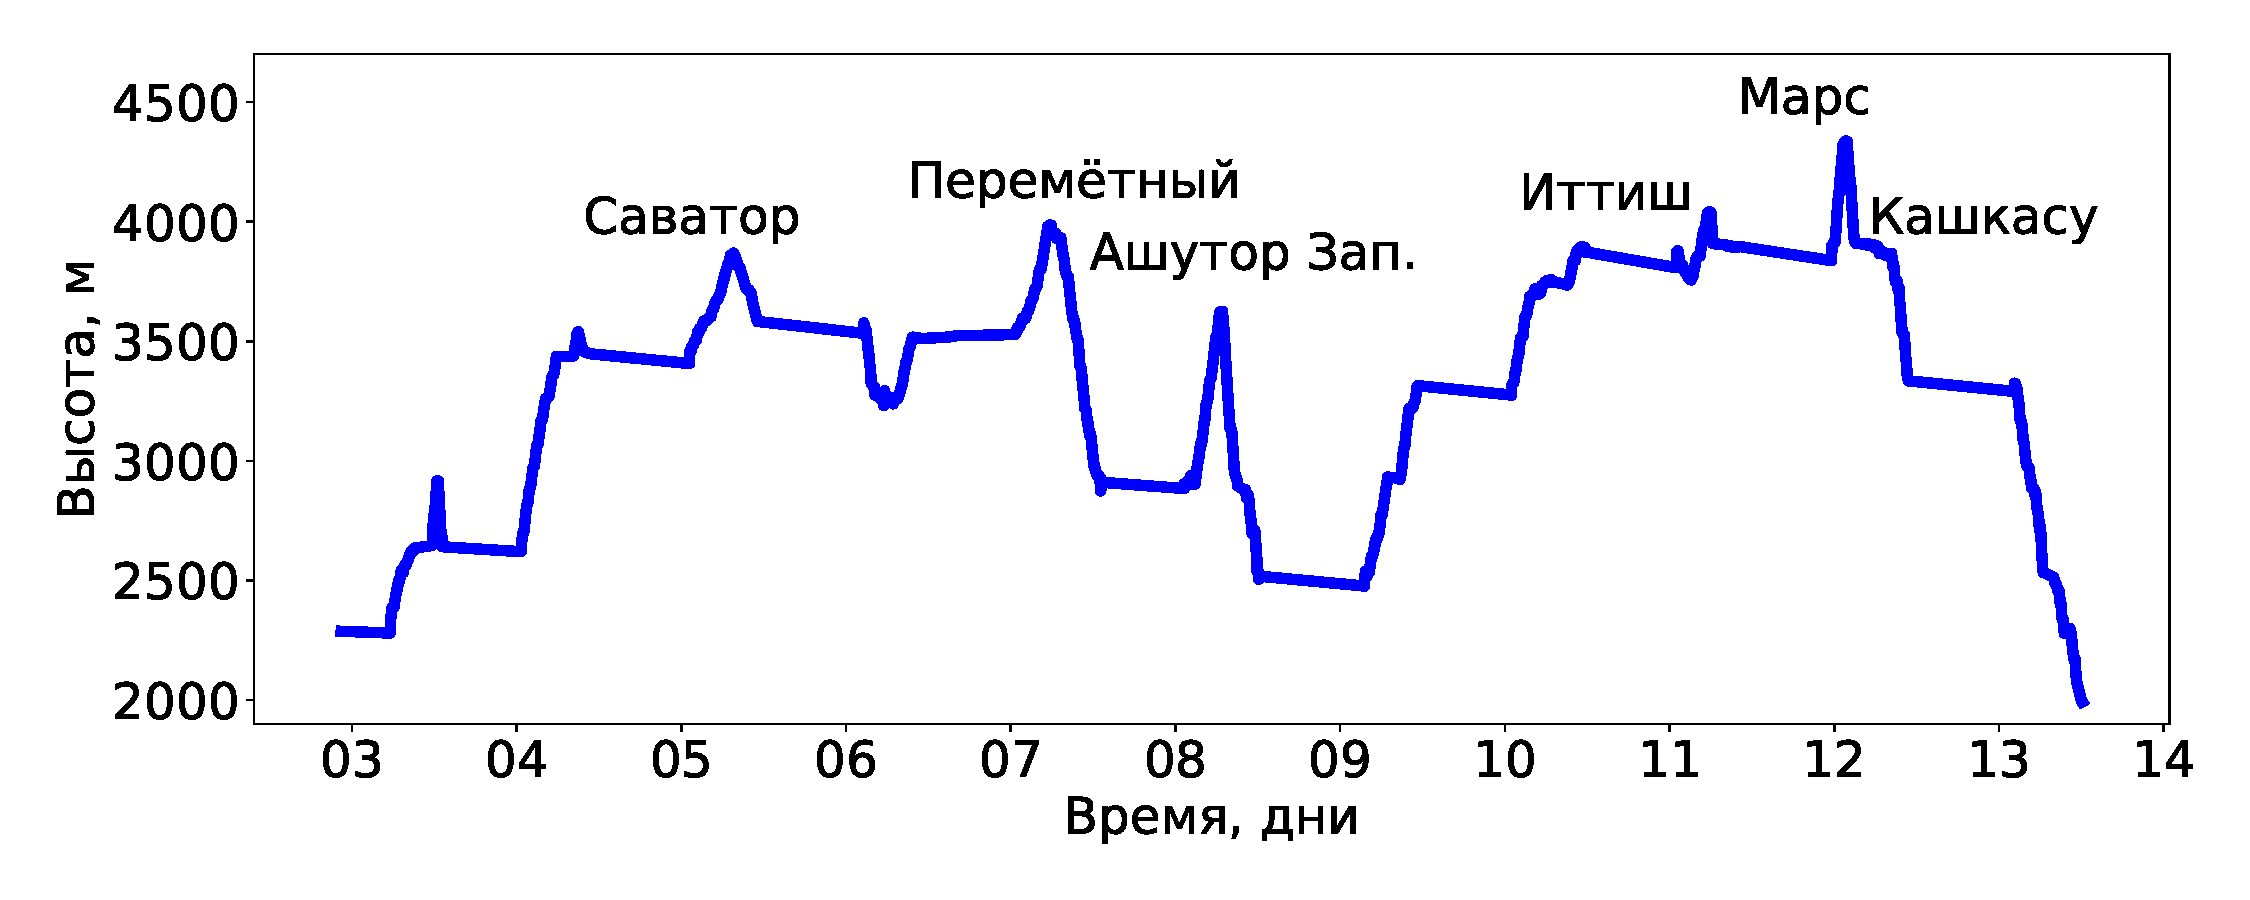
\includegraphics[width=0.92\linewidth]{elevation_vs_time}
	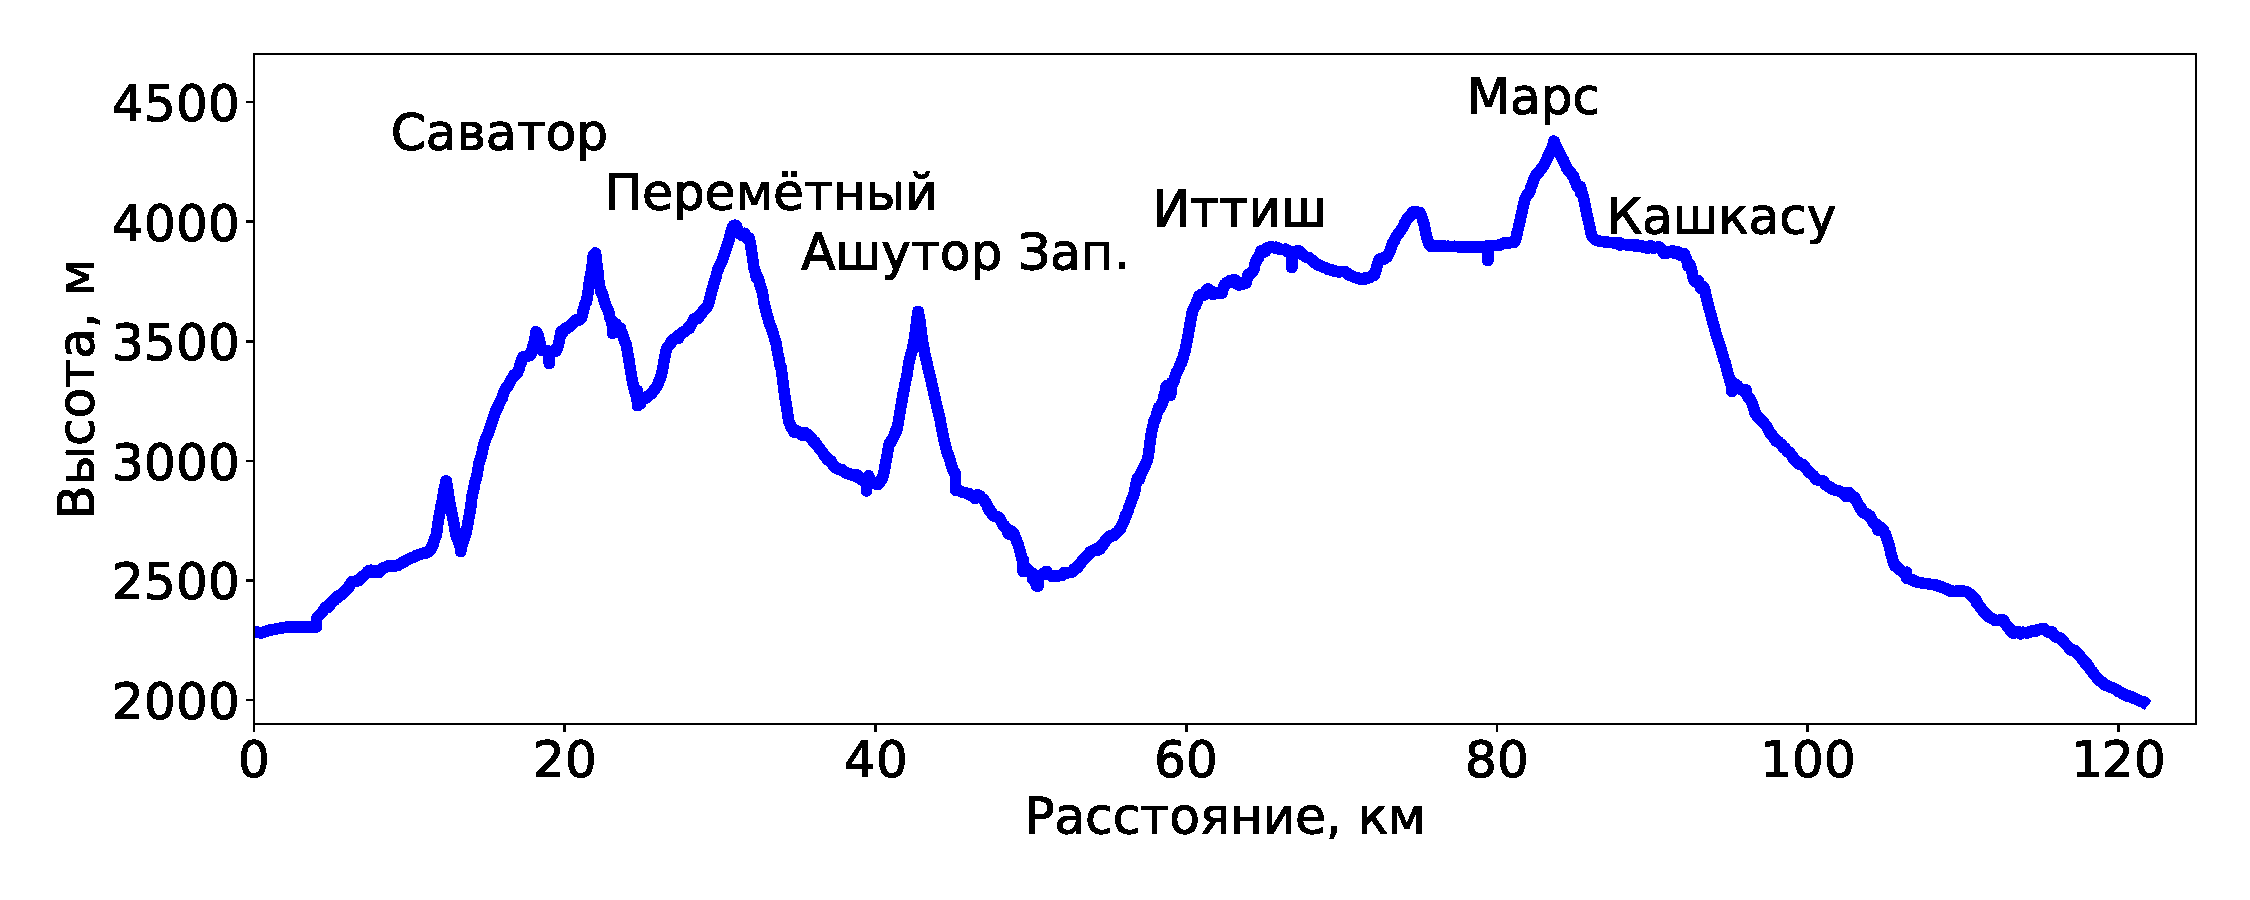
\includegraphics[width=0.92\linewidth]{elevation_vs_distance}
	\caption{Высотный профиль маршрута}
	\label{fig:heights}
\end{figure}

\newpage
\subsection{Определяющие препятствия маршрута}

\begin{table}[h!]
		\begin{tabular}{|>{\centering\arraybackslash}m{0.17\linewidth}|>{\centering\arraybackslash}m{0.03\linewidth}|>{\centering\arraybackslash}m{0.35\linewidth}|>{\centering\arraybackslash}m{0.35\linewidth}|}
			\hline
			\textbf{Вид препятствия, высота} &
			\begin{turn}{90}\textbf{к. тр.}\end{turn} &
			\textbf{Характеристика препятствия на подъём} &
			\textbf{Характеристика препятствия на спуск} \\
			\hline			
			пер. Саватор (4000, по GPS~--- 3860) & 1А &  Со стороны д.р. Саватор тр.-ос. перевальный взлёт протяжённостью до 400 м и крутизной до $30^{\circ}$.  & Со стороны д.р. Киче-Кызыл-Суу ск.-ос., движение до $25^{\circ}$ и протяжённостью до 200 м по крупной и средней осыпи крутизной плотной группой, самостраховка ледорубами, далее~--- по гребню морены и моренному карману.\\
			\hline			
			пер. Перемётный, (4026)  & 1А & Со стороны д.р. Киче-Кызыл-Суу движение по моренному лабиринту, далее по моренным гребням выход на левый пхд борт ледника. Перемётный ледник длиной 1200 м и крутизной  до $15^{\circ}$, движение без кошек. & Движение по перемётному леднику до 300 м  крутизной  до $15^{\circ}$, далее по моренным валам, траверс мелкоосыпного склона протяжённостью до 2 км и крутизной  до $20^{\circ}$ \\
			\hline
			пер. Ашутор Западный (3700)  & 1А & Со стороны д.р. Джукучак по тр.-ос. склону по руслу пересохшего ручья протяжённостью до 300 м, крутизной до $15^{\circ}$, на перевальном взлёте до до $25^{\circ}$. & Движение по границе белой и чёрной мелких осыпей, далее по руслу пересохшего ручья протяжённостью до 150 м., крутизной до $20^{\circ}$\\
			\hline
			пер. Иттиш, (3895)  & 1А & Со стороны д.р. Иттиш движение по ос. гребню протяженностью до 700~м крутизной  до $15^{\circ}$ & Движение по тр. склону протяжённостью до 1000 м и крутизной до $5^{\circ}$\\
			\hline
			пер. Кашкасу, (3890)  & 1А & Со стороны озёр Кашкасу движение по дну ущелья протяжённостью до 2500 м без значительного уклона. &  Движение по гребням морен протяжённостью до 3500 м и уклоном до $15^{\circ}$\\
			\hline
	\end{tabular}%
\end{table}

\clearpage
\subsection{Список участников} 

\begin{table}[h!]
	\centering
	\resizebox{0.8\textwidth}{!}{%
	\begin{tabular}{|>{\centering\arraybackslash}m{0.015\linewidth}|>{\centering\arraybackslash}m{0.14\linewidth}|>{\centering\arraybackslash}m{0.18\linewidth}|>{\centering\arraybackslash}m{0.05\linewidth}|>{\centering\arraybackslash}m{0.15\linewidth}|>{\centering\arraybackslash}m{0.3\linewidth}|}
		\hline
		\textbf{№} &
		\textbf{Фото} &
		\textbf{ФИО} &
		\textbf{г.р.} &
		\textbf{Обязанности в группе} &
		\textbf{Туристский опыт} \\
		\hline			
		
		1	&	\includegraphics[width=0.99\linewidth]{//webdav.cloud.mail.ru@SSL/DavWWWRoot/portraits/oa.jpg}	& Остапив Алексей Юрьевич	&	1998	&	Руководитель	& 2ГУ, Киргизский хребет,\newline 3$\times$1ГУ, Кавказ, Алтай \newline 2А тур., 1Б альп.\\
		\hline
		2	& \includegraphics[width=0.99\linewidth]{//webdav.cloud.mail.ru@SSL/DavWWWRoot/portraits/dd.jpg}	&Демушкин Дмитрий Юрьевич	&	2001	&	Штурман	& 1ГУ, Кавказ \newline 1А тур.\\
		\hline
		3	&	\includegraphics[width=0.99\linewidth]{//webdav.cloud.mail.ru@SSL/DavWWWRoot/portraits/mg.jpg}	&	Герасимова Мария Алексеевна	&	1981	&	Медик	&	\alert{1ГР Кавказ, 2ГУ Кавказ, 1ПУ Крым \newline 1Б тур.} \\
		\hline
		4	&		\includegraphics[width=0.99\linewidth]{//webdav.cloud.mail.ru@SSL/DavWWWRoot/portraits/ab.jpg}		&	Баранов Андрей Игоревич	&	1989	&	Финансист	&	1 ст.с., Кавказ \\
		\hline
		5	&	\includegraphics[width=0.99\linewidth]{//webdav.cloud.mail.ru@SSL/DavWWWRoot/portraits/ar.jpg}	&	Рогозин Александр Викторович	&	1996	&	Снаряженец	&	1 ст.с. Подмосковье \newline 2Б альп.\\
		\hline
		6	&	\includegraphics[width=0.99\linewidth]{//webdav.cloud.mail.ru@SSL/DavWWWRoot/portraits/yuz.jpg}	&	Зернина Юлия Алексеевна	&	2004	&	Завхоз	&	1 ст.с.  Кавказ\\
		\hline
		7	&	\includegraphics[width=0.99\linewidth]{//webdav.cloud.mail.ru@SSL/DavWWWRoot/portraits/ak.jpg}	&	Козлов Андрей Викторович	&	2004	&	Реммастер	&	1 ст.с. Подмосковье\\
		\hline
		8	&	\includegraphics[width=0.99\linewidth]{//webdav.cloud.mail.ru@SSL/DavWWWRoot/portraits/in.jpg}	&	Никитин Иван Сергеевич	&	2004	&	Фотограф	&	1 ст.с. Подмосковье\\
		\hline
	\end{tabular}%
	}
\end{table}

\clearpage

\subsection{Географическое положение района}

Район Тескей-Ала-Тоо (кырг. <<Пёстрые горы, обращённые от солнца>>)~--- это горный хребет, вхродящий в горную страну Центрального Тянь-Шаня. Тескей расположен к югу от озера Иссык-Куль, простираясь с запада на восток на 375 км. Средняя высота хребта около 4500 м, высшая точка достирает 5216 м (пик Каракольский).

Крупные узлы оледеления расположены в верховьях рек Чон-Кызылсуу, Джеты-Огуз, Каракол, Арашан, Ак-Суу и Тургень-Ак-Суу. В целом степень оледеления обусловлена высотой и наличием влажного воздуха от Иссык-Куля.

При движении с запада на восток среднегодовое количество осадков увеличивается вдвое, с 1000 мм до 2000 мм (для высокогорья) \cite{rodina2012}. Среднесуточная температура колеблется летом от -5\degree (сырты, высота 4000 м, август) до 15\degree~(д.р. Джукучак, высота 2500 м, август)

В районе ярко выражена высотная поясность. Зона леса, представленная преимущественно высокими тянь-шаньскими елями, располагается на высотах 2100--3100 м. До высоты 3800 м следует зона альпийских лугов, а снеговая линия в августе находится на высотах от 4000 м (для северных склонов хребта). Южная же сторона хребта представлена заболоченным плоскогорьем~--- сыртами, и как по климату, так и по растительности и рельефу резко контрастирует с северной стороной.

Долины рек, текущих вдоль отрогов главного хребта, широкие, долины их боковых притоков узкие с высокой и крутой устьевой ступенью.

\subsection{Туристские особенности района}
Район очень привлекателен для горных туристов, поскольку в нём представляется возможным проведение горных походов любой к.с.~--- от <<единичек>> до <<шестёрок>>. Этому способствуют несколько факторов: достаточно простая логистика, наличие локальных препятсивий любого уровня сложности в достаточном количества, разнообразие природного рельефа. Уникальной особенностью западной оконечности центрального Тескея (долины рек Джууку, Иттиш, Ашукашкасу, Джукучак) является возможность перехода с северной стороны хребта на южную по перевалам с категорией сложности не выше 1А, чем строго рекомендуется пользоваться при планировании простых горных походов по району.

Самыми посещаемыми долинами являются д.р. Чон-Кызыл-Суу, Джеты-Огуз, Телеты, Каракол. Здесь, помимо спортивных, проходит множество коммерческих маршрутов, можно встретить туристов из Европы и США. Прочие долины, несмотря на хорошую изученность, посещаются значительно реже. Впрочем, стоит отметить сильно возросший интерес к д.р. Джууку, Иттиш, Ашукашкасу, Джукучак после публикации отчёта Д. Ковинова в 2021 году \cite{kovinov2021}.

К дополнительным особенностям района стоит отнести наличие горячих радоновых источников в д.р. Джеты-Огуз, Джукучак, \alert{где-то ещё}

Типичной погодой для района следует считать ясную теплую первую половину дня и дождливый вечер (как правило, после 15:00) \cite{rodina2012, tipsina2024, sergeev2024, smurov2024}. Это следует обязательно учитывать при планировании ходового дня.

Все долины крупных рек, а также значительная часть их больших боковых притоков используются под высокогорных пастбища со всеми вытекающими последствиями для качества сырой воды.

\clearpage
\section{Организация и проведение похода}
\subsection{Цели и задачи маршрута. Выбор нитки маршрута}
При разработке и планировании маршрута я, как руководитель, руководствовался следующими соображениями:
\begin{enumerate} 
	\item \textbf{Высотность, транспортная доступность горного района и стоимость трансфера.}
	Подавляющая часть группы (шесть человек из восьми) имела официальный или неофициальный опыт горных походов до 2 к.с по Кавказу \cite{Snegovskaya2024} или Алтаю, и вся группа имела высотный опыт ночёвки не менее 2900 м \cite{ostapiv2025}. Это позволило выбрать в качестве района новичкового похода не Гвандру или Архыз, как это обычно бывает, а новый для участников и руководителя горный район Центральной Азии~--- Тескей-Ала-Тоо. Высоты в этом районе, в среднем, на 500 м больше, чем на Кавказе, а его транспортную доступность можно назвать приемлемой для новичковых походов: 4 часа самолётом до Бишкека и еще 7~--- до места старта в горах. Стоимость трансфера выше, чем на Кавказе, но ниже, чем на Алтае. 
		
	\item \textbf{Концентрированность препятствий.}
	Дополнительным фактором в сторону выбора Тескей-Ала-Тоо послужило также и то, что в отличие, например, от Алтая, хребтовка района (основной хребет и серия параллельных отрогов), как и на Кавказе, позволяет осуществить подход под многие перевалы в течение одного дня, миновав долгие и занудные забеги по долинам, и, как следствие, поддерживать интерес группы на приемлемом уровне.
	
	\item \textbf{Разнообразие рельефа.} 
	С методической точки зрения, а также, опять-таки, для поддержания интереса группы, хотелось продемонстрировать участникам как можно больше разнообразных типов рельефа. Район позволяет в походах 1 к.с. продемонстрировать все виды рельефа, за исключением, пожалуй, снежного. <<Изюминкой>> района является возможность пересечения главного хребта через перевалы 1А (разительно отличающихся от классических <<единичек А>>) с осмотром высокогорных болот~--- сыртов.
	
	\item \textbf{Эффект кульминации.}
	У меня как у руководителя было глубокое убеждение, что первый поход должен обладать понятным, с позволения сказать, сюжетом и иметь свою кульминацию. В нашем случае таким сюжетом было движение через отроги главного хребта с преодолением разнообразных перевалов (последовательно: травянисто-осыпной, ледовый, травянистый), а затем~--- кольцо через главный хребет с <<неклассическими>> перевалами на южную сторону, восхождением на обзорную точку~--- вершину Марс. Конец маршрута~--- забег по среднегорью с финишем на локальной достопримечательности <<Красные скалы>>~--- также должен был добавить в поход разнообразия и красоты. Наконец, по моему глубокому убеждению, финальным аккордом походов по Кыргызстану должен быть хотя бы  однодневный (а лучше двухдневный) отдых на Иссык-Куле.
	
	\item\textbf{Помощь в планировании}
	Фактор, который формально не был в списке определяющих критериев, но по факту являлся таковым~--- это искренняя заинтересованность и помощь в планировании и организации маршрута от человека, через которого организовывалась логистика похода~--- Юрия Траченко. За эту помощь выражаю ему огромную благодарность.
	
\end{enumerate} 
\subsection{Логистика}
Подъезд осуществлён на поезде 033М Москва--Владикавказ до станции Минеральные Воды (прибытие в 03:40). Стоимость проезда на август 2024 г. составляла 7800~\faRub, купе (обратно – 4700~\faRub, плацкарт). От Минеральных Вод до аула Верхний Учкулан (время в пути 4 часа) добирались на трансфере, заказанном через Саракуева Бориса (89289503868, 89298843175,  \href{mailto: bezonec@list.ru}{bezonec@list.ru}). Стоимость трансфера трансфера туда составила 18000~\faRub, обратно (от поляны Азау) — 15000~\faRub. Стоимости доставки забросок в т/б Глобус и а/л Узункол составили 4000~\faRub~и 6000~\faRub.
Коллективный пропуск в пограничную зону КЧР был оформлен за 4 месяца до начала похода через электронную почту пограничного управления ФСБ по КЧР~--- \href{mailto: pu.kcherkes@fsb.ru}{pu.kcherkes@fsb.ru} и отправлен письмом по указанному адресу. Пропуск в КБР не требуется, так как пер. Хотютау в 2023 году был исключён из пограничной зоны \cite{order_kbr}.
\subsection{Аварийные выходы из маршрута и его запасные варианты}
\textbf{Аварийными выходами} с маршрута являлись:
\begin{itemize}
	\item На первом этапе: спуск к т/б <<Глобус>>;
	\item На втором этапе: спуск к а/л <<Узункол>>;
	\item На третьем этапе: спуск к погранзаставе <<Актюбе>> (Хурзук).
\end{itemize}
\textbf{Запасными вариантами} маршрута являлись:
\begin{itemize}
	\item Замена пер. Уллу-Кёль Восточный (1А$^\star$, 3050) на пер. \textbf{Уллу-Кёль Нижний (н/к, 2933)};
	\item Отказ от пер. Перемётный (1А, 3255), спуск по д.р. Чунгур-Джар;
	\item Отказ от пер. Хотютау (1А$^\star$), спуск по д.р. Кубань к погранзаставе <<Хурзук>>
\end{itemize}
\subsection{Изменение маршрута и их причины}
Маршрут пройден без изменений.
\subsection{Обеспечение безопасности на маршруте}
Группа была зарегистрирована в отделении МЧС Кыргызстана по Иссык-Кульской области (телефон +996555004214, связь по WhatsApp). За 10 дней до похода были переданы сведения о составе группы, сроках и маршруте, в ответ был получен регистрационный номер и просьба проинформировать дежурного о начале и завершении похода.

\alert{Дима, это с тебя Для регулярного обмена сообщениями, отслеживания положения группы на карте, а также возможности экстренной связи, в группе имелся спутниковый треккер IRIDIUM Rockstar 360. Стоимость аренды треккера в <<Альпиндустрии>> на 15--21 день составила 7100~\faRub, залог~--- 50000~\faRub. Нам повезло попасть на демострационный период тарифа треккера, в связи с чем все сообщения были для нас безлимитны и бесплатны. Предварительное тестирование треккера в Москве показало, что спутниковые сигналы в столице эффективно глушатся: сообщения приходили не чаще раза в сутки. В походе с приёмом и отправкой сообщений и координат на сервер проблем не возникало, среднее время отправки составляло 30 минут.}

Каждый участник самостоятельно оформлял на себя индивилуальный страховой полис. Выбрали страховую фирму <<Согласие>>, ассист Balt Assistance, опция <<Треккинг свыше 1500 м>>, размер страховой защиты 35000~USD,  вид отдыха <<Спорт Экстрим>>. Стоимость полиса составила 8234~\faRuble~с человека.

\subsection{Перечень наиболее интересных природных и исторических объектов, занятий на маршруте}
\begin{enumerate}[noitemsep,topsep=0pt,parsep=0pt,partopsep=0pt]
	\item Широкие красивые долины северной стороны хребта: Чон-Кызыл-Суу, Киче-Кызыл-Суу, Ашукашкасу, Джукучак; 
	\item Сырты на южной стороне хребта; 
	\item Цепочка озёр Кашкасу с чистой водой; 
	\item Вершина Марс, с которой открываются виды на Акширак, Кумтор, сырты и, в хорошую погода, на семитысячники; 
	\item Перевал Кашкасу, через который в былые годы перегоняли лошадей. Следы этого остаются в ущелье до сих пор, жутковато и атмосферно; 
	\item <<Красные скалы>> на слиянии р. Джууку и Джукучак;
	\item Иссык-Куль.
\end{enumerate}

\paragraph{Темы практических занятий:}

\begin{itemize}
	\item Техника передвижения по травянисто-осыпным склонам;
	\item Техника передвижения по снегу, льду.
\end{itemize}

\newpage
\subsection{Развёрнутый график движения}
\begin{table}[h!]
	\centering
	\resizebox{0.95\textwidth}{!}{%
		\begin{tabular}{|>{\centering\arraybackslash}m{0.045\linewidth}
				|>{\centering\arraybackslash}m{0.02\linewidth}
				|>{\centering\arraybackslash}m{0.43\linewidth}
				|>{\centering\arraybackslash}m{0.09\linewidth}
				|>{\centering\arraybackslash}m{0.1\linewidth}
				|>{\centering\arraybackslash}m{0.05\linewidth}
				|>{\centering\arraybackslash}m{0.09\linewidth}
				|>{\centering\arraybackslash}m{0.13\linewidth}|}
			\hline						
			Дата	&	\begin{turn}{90}День\end{turn}	&	Участок маршрута	&	Км с $k=1.2$	&	Набор /сброс, м	&	ЧХВ	&	Высота ночёвки, м	&	Способы передвижения	\\
			\hline
			
			18.08	&	1	&	г.~Минеральные воды~--- аул Верхний Учкулан~--- д.р Учкулан~--- д.р. Кичкинакол Уллукёльский	&	5.3	&	$+650$\newline$-0$	& 2:46	&	2200	&	Машина,\newline Пешком	\\
			\hline
			19.08	&	2	&	д.р. Кичкинакол Уллукёльский~--- оз. Гитче-Кёль~--- оз. Уллу-Кёль 	&	5.6	& $+650$\newline$-0$		& 3:25		& 2850		&	Пешком	\\
			\hline
			20.08	&	3	&	м.н.~--- \textbf{пер. Уллу-Кёль Восточный (1А$^\star$, 3050)}~--- кош в д.р. Трёхозёрная~--- д.р. Махар	&	7.2	& $+200$\newline$-1190$		& 7:39	& 1860		&	Пешком	\\
			\hline
			21.08	&	4	&	м.н.~--- т/б <<Глобус>>~--- д.р. Гондарай~--- д.р. Джалпаккол	&	11.3	&$+390$\newline$-225$		& 3:54		& 2120		&	Пешком	\\
			\hline
			22.08	&	5	&	м.н.~--- д.р. Кичкинекол Джалпаккольский~--- м.н. под моренным валом пер. Джалпаккол Северный	&	5.8	& $+620$\newline$-0$		& 3:56	& 2740		&	Пешком	\\
			\hline
			23.08	&	6	&	м.н.~--- \textbf{пер. Джалпаккол Северный (1А$^\star$, 3411)}~--- зелёные ночёвки на спуске в д.р. Мырды	&	5.0 	& $+660$\newline$-395$		& 6:16		& 3015		&	Пешком	\\
			\hline
			24.08	&	7	&	м.н.~--- д.р. Мырды~--- а/л <<Узункол>>	&	7.5	& $+0$\newline$-960$		& 3:53		& 2060		&	Пешком	\\
			\hline
			25.08	&	8	&	м.н.~--- д.р. Кичкинекол~--- д.р. Таллычат~--- Поляна Крокусов	&	7.1	& $+780$\newline$-0$		& 3:23		& 2840		&	Пешком	\\
			\hline
			26.08	&	9	&	м.н.~--- \textbf{пер. Кичкинекол Малый (1А, 3206)}~--- д.р. Чунгур-Джар	&	4.6	& $+360$\newline$-520$		& 2:42		& 2680		&	Пешком	\\
			\hline
			27.08	&	10	&	м.н.~--- \textbf{пер. Перемётный (1А, 3255)}~--- д.р. Танышхан	&	7.1	& $+575$\newline$-935$		& 6:50		& 2320		&	Пешком	\\
			\hline
			28.08	&	11	&	м.н.~--- д.р. Чиринкол~--- д.р. Кубань &	12.7	& $+90$\newline$-500$		& 3:23		& 1890		&	Пешком	\\
			\hline
			29.08	&	12	&	м.н.~--- погранзастава <<Хурзук>>~(рад.)~--- д.р. Уллу-Кам	&	20.9	& $+1210$\newline$-370$		& 7:15		& 2725		&	Пешком	\\
			\hline
			30.08	&	13	&	м.н.~--- \textbf{пер. Хотютау (1А$^\star$, 3546)}~--- лед. Большой Азау~--- оз. Эльбрусское~--- ст. <<Старый Кругозор>>~--- поляна Азау & 10.9	& $+800$\newline$-615$		& 4:25		& 2915		&	Пешком, Канатная дорога	\\
			\hline
			\multicolumn{3}{|c|}{\textbf{\textit{\Large{Итого:}}}} & \large{\textbf{111.0}} & \large{$\mathbf{+6985}$\newline$\mathbf{-5210}$	}	& \multicolumn{3}{c|}{\large{\textbf{58:08}\newline\textbf{2д 10ч 08мин}}} \\
			\hline
		\end{tabular}
}	
	
\end{table}



\clearpage
\section{Литературный обзор по прохождению маршрута}

\subsection{Пер. Иттиш}

Пер. Иттиш ориентирован с севера на юг и является перевалом через основной хр. Тескей-Ала-Тоо. Это один из немногих перевалов через данный основной хребет, которые имеют (низкую) трудность 1А. Вообще говоря, пер. Иттиш~--- это выход на горизонтальное плато, на котором расположены сырты (заболоченные луга). Лишь северная сторона перевала имеет наклон. Ранее \alert{ссылка} перевал проходился на спуск с юга на север; в данном походе было решено преодолеть его на подъем с севера на юг. При подготовке использовались отчеты \alert{ссылки}.

Подъем на перевал можно разбить на две части: подъем по тропе по хвойному лесу и осыпи и горизонтальное движение по средней и крупной осыпи. Второй этап недлинный по расстоянию -- около 4-5 км -- но может занять много времени из-за трудности рельефа. В некоторых местах можно сойти с крупных камней и двигаться по пересохшему дну озер, находящихся вблизи осыпи. При подходе к седловине видно обледенелый пик Иттиш и ледник, примыкающий к нему. После взятия перевала спуска нет -- сразу идет выход на высокогорные сырты и озера. Также в хорошую погоду с седловины открывается вид на соседний хр. Акшийрак. В целом, подъем является постепенным и не имеет крутых взлетов.

Суммарный перепад высот от д.р. Джууку, из которой начинался подъем, до седловины перевала составляет около 1000м, поэтому было решено устроить ночевку в середине подъема на небольшом озере, находящимся выше границы леса. От м.н. ночевки на озере до седловины перевала был пройден остаток подъема по средней осыпи и затем преодолен упомянутый затяжной участок горизонтальной осыпи.

\clearpage
\section{Техническое описание маршрута}
%\textit{Примечание:} везде, если не оговорено иное, имеются в виду правые и левые берега рек \textbf{орографически}.

\textbf{Отчёт писали:} Даша Снеговская, Лёша Остапив, Даша Казаринова, Вика Суровцева, Дима Дёмушкин, Катя Тюрина, Илья Шалфеев, Дима Сингалевич.
\subsection{18 августа. Старт}
\textit{Метеоусловия: утром, днём, вечером ясно, тепло.}

\begin{figure}[h!]
	\centering
	\includegraphics[angle=0, width=0.7\linewidth]{../pics/mini_maps/18}
	\label{fig:mini_18}
\end{figure}

Прибыли в г. Минеральные Воды в 03:40. Встретились на вокзале с участником, прибывшим на день раньше, и загрузились в машину Бориса Саракуева. В 04:00 отправились на место старта (мост через р. Учкулан, N 43.38668\degree~E 41.98961\degree), куда прибыли в 09:45 (по дороге на 40 минут остановились в ауле Учкулан, чтобы позавтракать). Распределили заброски, отдали их водителю и выдвинулись на маршрут в 11:18. Первые 1.5 км до коша шли по д.р. Учкулан, затем тропа повела через калитку и повернула направо, на подъём в висячую долину р. Кичкинакол Джалпаккольский.

\begin{figure}[h!]
	\centering
	\includegraphics[width=0.7\linewidth]{../pics/DSC_0412}
	\caption{группа на старте маршрута в д.р. Учкулан}
	\label{fig:uchkulan}
\end{figure}

\begin{figure}[h!]
	\centering
	\includegraphics[width=0.7\linewidth]{../pics/DSC_0436}
	\caption{Подъём по тропе в д.р. Кичкинакол Уллукёльский}
	\label{fig:DSC_0436}
\end{figure}

Подъём здесь идёт по хорошей тропе со средним уклоном порядка 20\degree~ (рис.~\ref{fig:DSC_0436}). Шли не спеша, в режиме 20/5 и далее вплоть до 10/10, разгружая отстающих участников. В 14:30 завершили подъём в долину и устроили обед.

\begin{figure}[h!]
	\centering
	\includegraphics[width=0.7\linewidth]{../pics/DJI_0805}
	\caption{д.р. Кичкинакол Джалпаккольский}
	\label{fig:kichkinakol}
\end{figure}

С обедом закончили в 16:40 и прошли 2 км к оборудованной стоянке возле коша, где оказались в 17:25. Рядом местные жители собирали малину. Подумав немного и устроив разведку, поднялись ещё немного выше и в 18:18 встали на место ночёвки на оборудованной стоянке возле дерева на небольшом разливе реки. Координаты м.н. N 43.35392\degree~E 41.96858\degree.
\begin{figure}[h!]
	\centering
	\includegraphics[width=0.7\linewidth]{../pics/camp_18}
	\caption{Место ночёвки 18-19.08}
	\label{fig:camp_18}
\end{figure}

\clearpage
% \input{aug19}
% \input{aug20}
% \input{aug21}
% \input{aug22}
% \input{aug23}
% \input{aug24}
% \input{aug25}
% \input{aug26}
% \input{aug27}
% \input{aug28}
% \input{aug29}
% \input{aug30}
\section{Материальное обеспечение группы}

\begin{table}[h!]
	\centering
%	\resizebox{0.77\textwidth}{!}{%
		\begin{tabular}{|>{\centering\arraybackslash}m{0.02\linewidth}|>{\centering\arraybackslash}m{0.31\linewidth}|>{\centering\arraybackslash}m{0.08\linewidth}|>{\centering\arraybackslash}m{0.29\linewidth}|>{\centering\arraybackslash}m{0.08\linewidth}|}
			\hline
			\multirow{2}{*}{\textnumero}	&	\multicolumn{2}{|c|}{Личное}	&	\multicolumn{2}{|c|}{Специальное}	\\
			
			\cline{2-5} & Наименование	&	Кол-во	&	Наименование	&	Кол-во\\
			\hline
			1	&	Верёвка статическая 50~м, $\varnothing=9$~мм	&	1	&	Система с блокировкой	&	1	\\
			\hline
			2	&	Общественные карабины	&	5	&	Карабины	&	3	\\
			\hline
			3	&	Ледобуры	&	2	&	Спусковое устройство	&	1	\\
			\hline
			4	&	Станционные петли 180~см	&	3	&	Жумар	&	1	\\
			\hline
			5	&	Общественный корделет	&	2	&	Прусик короткий	&	2	\\
			\hline
			6	&	GPS-навигатор	&	1	&	Ледоруб	&	1	\\
			\hline
			7	&	Спутниковый треккер	&	1	&	Каска	&	1\\
			\hline
			8	&	&		&	Кошки	&	1 пара\\
			\hline
			9	&	&		&	Солнцезащитные очки	&	1\\
			\hline

		\end{tabular}%
%	}
\end{table}



\clearpage
\section{Финансовый отчёт}

\begin{table}[htbp]
	\centering

		\begin{tabular}{|>{\centering\arraybackslash}m{0.5\linewidth}
				|>{\centering\arraybackslash}m{0.2\linewidth}
				|>{\centering\arraybackslash}m{0.2\linewidth}|}
			
			\hline						
		Статья расхода	&	На группу,~\faRub	&	На человека,~\faRub	\\
		\hline
		Поезд Москва--Мин. Воды (купе)	&	93600 	&	7800	\\
		\hline
		Поезд Мин. Воды--Москва (плацкарт)	&	56400	&	4700	\\
		\hline
		Продукты по раскладке	&	66386	&	5533	\\
		\hline
		Газ	&	8400	&	700	\\
		\hline
		Трансфер и доставка забросок&	43000	&	3584	\\
		\hline
		Хранение забросок &	3000	&	250	\\
		\hline
		Ночёвка в а/л <<Узункол>>	&	5500	&	459	\\
		\hline
		Страховка	&	68600	&	5717	\\
		\hline
		Ремнабор	&	2340	&	195	\\
		\hline
		Аптечка	&	12089	&	1008	\\
		\hline
		Аренда общественного снаряжения	&	2900	&	242	\\
		\hline
		Аренда спутникового треккера	&	7100	&	592	\\
		\hline
		Прочее (баня в а/л <<Узункол>>)	&	2500	&	209	\\
		\hline
		\textbf{ИТОГО:}	&	\textbf{371815}	&	\textbf{30985}	\\
		\hline
		\end{tabular}
	
\end{table}



\newpage
\section{Итоги похода, выводы и рекомендации по совершённому походу (от лица руководителя)}

\subsection{Подготовка к походу и взаимодействие с группой} 
	\begin{enumerate}
		\item При подготовке участников особое внимание требуется уделить навыку подстраховки альпенштоком. В нашем случае ни у кого из участников не было проблем с движением по курумнику --- что можно считать большим везением --- и лимитирующим фактором для скорости группы становились именно крутые спуски, на которых большинство участников не смогло обеспечить себе уверенную страховку, потому что навык спуска с альпенштоком не был достаточно отработан; 
		\item Для некоторых участников хождение ночью с фонариком оказалось большим стрессом. Этот навык тоже следует отрабатывать отдельно на разного рода ночных ориентированиях при подготовке к походу; % \st{В смысле, не ходить ночью? Не, фигня!}
		\item Долгие утренние сборы в походе были организационной ошибкой руководителя. Предположительно, сборы можно было ускорить, причём, по отзывам участников, без особых усилий с их стороны; 
		\item В походе, в начале каждого дня участникам не хватало озвучивания плана на день, а непосредственно на марше~--- коммуникации руководителя с участниками; 
		\item При подготовке хотелось бы большей автоматизации при расчёте весов и учёте снаряжения --- работу с гугл-доком следует оптимизировать.
	\end{enumerate} 
	
\subsection{Выбор и прохождение маршрута}  
	\begin{enumerate}
		\item Решение провести поход в конце августа я оцениваю в конечном итоге как разумное, хотя не все ожидания оправдались. А именно, с точки зрения погоды на маршруте --- по моим личным ощущениям ---конец августа не сильно выигрывает у конца июля -- начала августа: также не редки грозы и дожди. Тем не менее, благодаря поздним срокам была достаточная уверенность в том, что лед. Большой Азау окажется открытым --- и эти ожидания оправдались --- а также скорее повезло с состоянием снега на пер. Уллу-Кёль Восточный. По информации, полученной нами от руководителя похода 1 к.с., Антона Колотова, в том же районе, но в июле, на Уллу-Кёле Восточном может быть снежный карниз.
		\item Упомянутый выше перевал Уллу-Кёль Восточный при том количестве снега, которое было в нашем случае, и при тех условиях, на мой взгляд, проходим, но только при условии наличия кошек у всей группы. Также вызывает вопрос наилучшая техника его прохождения: стоит ли в конце подъёма ставить кошку боком на всю ступню или идти на три такта, если снег раскис; 
		\item Насчёт кошек: моё мнение было и остаётся таким, что на данном маршруте кошки строго необходимо иметь всем участникам группы из-за перевалов. Уллу-Кёля Восточного и Джалпаккола Северного; 
		\item Спуск с пер. Перемётного на 900 м по высоте вместо 300 был явной ошибкой руководителя и штурмана; 
		\item Тем не менее, само прохождение пер. Перемётного и спуск в д.~р. Чиринкол по левому берегу р. Таллычат я оцениваю скорее как удачное решение; 
		\item В целом, пройденная нами нитка маршрута, за исключением, возможно, пер. Уллу-Кёль Восточный, видится мне эталонной и отвечает всем заявленным требованиям для горного маршрута 1 к.~с., особенно, если для многих участников этот поход является первым. Пер. Уллу-Кёль Восточный, возможно, имеет смысл заменить на пер. Уллу-Кёль Нижний, но до конца я в этом не уверена; 
	\end{enumerate}
	\clearpage
\appendix

%\section{Перевальные записки}

\begin{figure}[h!]
	\begin{minipage}[h!]{0.49\linewidth}
		\centering{\includegraphics[width=0.98\linewidth]{../pics/notes/ullukuel_front}}
	\end{minipage}
	\hfill
	\begin{minipage}[h!]{0.49\linewidth}
		\centering{\includegraphics[width=0.98\linewidth]{../pics/notes/ullukuel_rev}}
	\end{minipage}
	\caption{Записка с пер. Уллу-Кёль Восточный}
	\label{pic:ullu_kuel}
\end{figure}

\begin{figure}[h!]
	\begin{minipage}[h!]{0.325\linewidth}
		\centering{\includegraphics[width=0.98\linewidth]{../pics/notes/dzhalpakkol1_front}}
	\end{minipage}
	\hfill
	\begin{minipage}[h!]{0.325\linewidth}
		\centering{\includegraphics[width=0.98\linewidth]{../pics/notes/dzhalpakkol1_rev}}
	\end{minipage}
	\hfill
	\begin{minipage}[h!]{0.325\linewidth}
		\centering{\includegraphics[width=0.98\linewidth]{../pics/notes/dzhalpakkol2_front}}
	\end{minipage}
	\caption{Записки с пер. Джалпаккол Северный}
	\label{pic:dzhalpakkol}
\end{figure}

\begin{figure}[h!]
	\begin{minipage}[h!]{0.49\linewidth}
		\centering{\includegraphics[width=0.7\linewidth]{../pics/notes/kichkinekol_front}}
	\end{minipage}
	\hfill
	\begin{minipage}[h!]{0.49\linewidth}
		\centering{\includegraphics[width=0.7\linewidth]{../pics/notes/kichkinekol_rev}}
	\end{minipage}
	\caption{Записка с пер. Кичкинекол Малый}
	\label{pic:kichkinekol}
\end{figure}

\begin{figure}[h!]]
	\centering{\includegraphics[width=0.7\linewidth]{../pics/notes/peremetnyy_front}}
	\caption{Записка с пер. Перемётный}
	\label{pic:peremetnyy}
\end{figure}

\begin{figure}[h!]
	\begin{minipage}[h!]{0.325\linewidth}
		\centering{\includegraphics[width=0.98\linewidth]{../pics/notes/hotyutau1_front}}
	\end{minipage}
	\hfill
	\begin{minipage}[h!]{0.325\linewidth}
		\centering{\includegraphics[width=0.98\linewidth]{../pics/notes/hotyutau2_front}}
	\end{minipage}
	\hfill
	\begin{minipage}[h!]{0.325\linewidth}
		\centering{\includegraphics[width=0.98\linewidth]{../pics/notes/hotyutau2_rev}}
	\end{minipage}
	\caption{Записки с пер. Хотютау}
	\label{pic:hotyutau}
\end{figure}
\clearpage


\printbibliography



\end{document}